\documentclass[conference]{IEEEtran}
\usepackage[margin=1in]{geometry}
\usepackage{cite}
\usepackage{amsmath,amssymb,amsfonts}
\usepackage{algorithmic}
\usepackage{graphicx}
\usepackage{textcomp}
\usepackage{xcolor}
\usepackage{subcaption}
\usepackage{cuted}

\title{A Steady State Model for the Continuous Conversion Ratio Charge Pump}

\begin{document}
	\maketitle
	\section{Introduction}
	The rise of IoT has driven the development of various ultra low power, low cost mobile systems. This results in a need for high efficiency, low cost power electronics.
	
	One extremely promising candidate for addressing many of the needs of industry is the continuously scalable charge pump proposed in \cite{Butzen2019	}. The proposed structure has the benefit of providing a completely variable conversion ratio while maintaining high efficiencies. 
	
	The development of models for the structure will facilitate reduced design times, and a more streamlined design flow. One of the important aspects of the continuous ratio converter is the resulting impact of incomplete charge transfer on the efficiency and performance of the converter. The following work proposes a steady state model that will incorporate the effects of incomplete charge transfer into the existing equations for input and output current.
	
	The structure of the paper is as follows, first, a model of the charge pump will be generated. Next, the results of the model are then compared to simulations performed in LTspice. The results are then discussed, along with the validity of the assumptions.
	\section{Steady State Model}
	The circuit to be analyzed is the continuous conversion ratio circuit as seen in \cite{Butzen2019}, which can be seen in Fig. \ref{fig:contTop}. The various steps are numbered along with their associated capacitors in Fig. \ref{fig:contTop}, and will be used further in the analysis. The circuit diagram corresponding to a single flying capacitor and its switches (also referred to as a "core") can be seen in Fig. \ref{fig:coreCon}. The analysis and modeling is performed under the following assumptions,
	\begin{itemize}
		\item All the capacitors are linear.
		\item The top and bottom plate parasitic capacitance's have minimal impact on the transient and steady state characteristics of the converter, and are neglected from the analysis.
		\item All the flying capacitors are equally sized with capacitance $C_{Fly}$, where $C_{Fly} = C_{1,0} = C_{1,1} = C_{2,0} = C_{2,M} ...$
		\item The switches for the intermediary nodes, $S_{T1}, S_{T2}, S_{TM}, S_{B1}, S_{BN}, etc$, all have an equivalent resistance $R_{ON}$. The resistance of the switches which connect to the positive and negative rails is 0$\Omega$ ($S_{T+}, S_{T-}, S_{B+}, S_{B-}$).
	\end{itemize}
	\begin{figure}
		\centering
		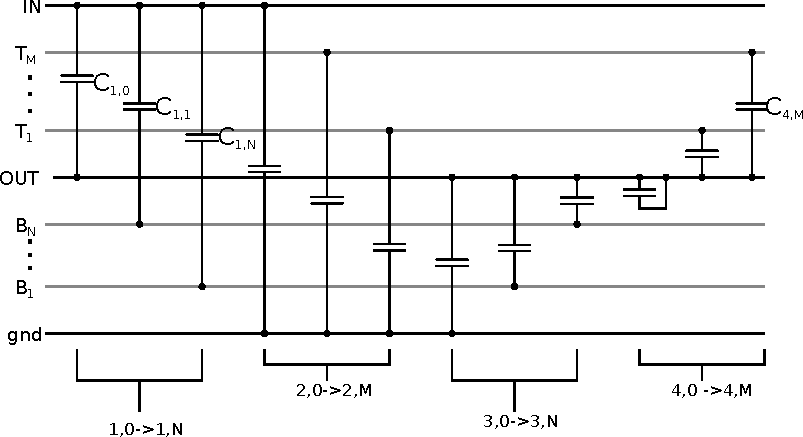
\includegraphics[width=\linewidth]{Figures/contRatioCircuit2.pdf}
		\caption{Circuit diagram illustrating the various connections made by the flying capacitors for the continuous ratio.}
		\label{fig:contTop}
	\end{figure}
	\begin{figure}
		\centering
		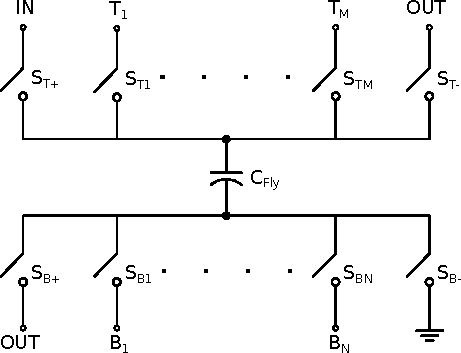
\includegraphics[width=0.8\linewidth]{Figures/contRatioCore.pdf}
		\caption{Circuit diagram illustrating the top and bottom connections of a single flying capacitor.}
		\label{fig:coreCon}
	\end{figure}
	\subsection{Charge Transfer Analysis}
	The operation of the converter is as follows, each capacitor iterates from steps (1,0)$\rightarrow$(4,M) sequentially. There is always a connection on the top or bottom plate to either 0$\,$V, $V_{IN}$ or $V_{OUT}$. The other connection to the intermediary voltage domains (those being $B_1 \rightarrow B_N$ and $T_1 \rightarrow T_M$) occurs through a switch with a resistance $R_{ON}$, where the core voltage begins to equalize with the new voltage domain. An example circuit can be seen in Fig. \ref{fig:step_Circ1}, which is electrically equivalent to Fig. \ref{fig:step_Circ2}. 
	
	\begin{figure}
		\centering
		\begin{subfigure}{0.4\textwidth}
			\centering
			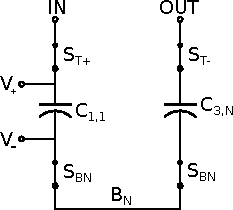
\includegraphics{Figures/step2_Circ.pdf}
			\caption{Circuit configuration including switches and flying capacitors.}
			\label{fig:step_Circ1}
		\end{subfigure}
		\begin{subfigure}{0.4\textwidth}
			\centering
			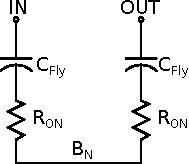
\includegraphics{Figures/step2_Eq.pdf}
			\caption{Equivalent circuit with values.}
			\label{fig:step_Circ2}	
	\end{subfigure}
		\caption{Example circuit diagrams showing the connection to $B_1$.}
	\end{figure}

	\begin{figure}
		\centering
		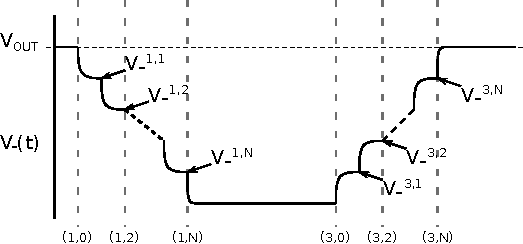
\includegraphics[width=0.9\linewidth]{Figures/V-(t).pdf}
		\caption{Illustration of $V_{-}(t)$ for various time steps over the period, where $V_-$ is the bottom plate of the capacitor, as in \ref{fig:step_Circ1}.}
		\label{fig:V-(t)}
	\end{figure}
	
	The circuit diagram in Fig. \ref{fig:step_Circ2}, can be used to calculate the transient response of the circuit over each time step. Consider node ($B_N$),  the impedance of both branches to IN and OUT is identical, this symmetry results in $B_N$ being constant over a single time step. The top and bottom plate voltages of the capacitors can then be described using a single $RC$ time constant ($\tau$), where $\tau = R_{ON}C_{Fly}$. Using Fig. \ref{fig:step_Circ2} as an example, the top plate voltage of $C_{1,1}$ is known, while the bottom plate voltage ($V_{-}^{1,1}$) can be calculated as,
	\begin{equation}
	V_{-}^{1,1}(t) = V_{OUT}\exp\left(\frac{-t}{\tau}\right) + V_{BN}\left(1-\exp\left(\frac{-t}{\tau}\right)\right),
	\end{equation}
	where $t$ is the time after the start of the step. More generally, the top and bottom plate voltages can be described as,
	\begin{equation}
	V_{C}[n]\! =\! V_{C}[n\!-\!1]\exp\left(\tfrac{-1}{\tau f_{SW}}\right) + V_{int}\!\left(1-\exp\left(\tfrac{-t}{\tau f_{SW}}\right)\right),
	\label{eq:Vstepn}
	\end{equation}
	where $V_{C}[n-1]$ is the voltage at the end of previous step, while $V_{int}$ is the voltage of the intermediary node ($V_{T1}$, $V_{TM}$, $V_{B1}$, etc) which the capacitor is connected to. Next, the duration of each time step can be incorporated into the analysis using the switching frequency ($f_{SW}$). A substitution can then be made to simplify the analysis, where
	\begin{equation}
	A = 1-\exp\left(\frac{-1}{\tau f_{SW}}\right),
	\end{equation}
	which can be substituted into (\ref{eq:Vstepn}) for example
	\begin{equation}
		V_{C}[n] = V_C[n-1]A + V_{int}(1-A),
	\end{equation}
	which can then be used to express the bottom plate voltage as a series of multiplications. The bottom plate voltage for steps (1,1)$\rightarrow $(1,N) is illustrated in Fig. \ref{fig:V-(t)}, and can be described as a sequence of transitions, where
	\begin{equation}
	\begin{split}
	V_-^{1,1} &= V_{OUT}(1-A) + AV_{BN},\\
	V_-^{1,2} &= V_-^{1,1}(1-A) + AV_{BN-1},\\
	& \,\,\,\vdots\\
	V_{-}^{1,N} &= V_-^{1,N-1}(1-A) + AV_{B1}.
	\end{split}		
	\end{equation}
	Using this, the matrix in equation (\ref{eq:V_1}) can be constructed to describe the bottom plate voltages.
\begin{figure*}
		\begin{equation}
	\begin{split}
	\begin{bmatrix}
	V_-^{1,1} \\
	V_-^{1,2} \\
	\vdots\\
	V_-^{1,N-1} \\ 
	V_-^{1,N}
	\end{bmatrix}
	&\!=\!
	\begin{bmatrix}
	A \!& 0 & \dots & 0 & 0 \\
	A(1-A) \!& A & \dots & 0 & 0\\
	\vdots & \vdots & \ddots & \vdots & \vdots \\
	A(1\!-\!A)^{N-2} \!& A(1\!-\!A)^{N-3} \!& \dots & A & 0\\ 
	A(1\!-\!A)^{N-1} \!& A(1\!-\!A)^{N-2} \!& \dots & A(1-A) & A 
	\end{bmatrix}\!\begin{bmatrix}
	V_{BN} \\
	V_{BN-1} \\
	\vdots \\
	V_{B2} \\
	V_{B1}
	\end{bmatrix}+V_{OUT}\begin{bmatrix}
	(1-A) \\
	(1-A)^2 \\
	\vdots \\
	(1-A)^{N-1} \\
	(1-A)^N
	\end{bmatrix}
	\end{split}
	\label{eq:V_1}
	\end{equation}
\end{figure*}
	Using a similar method, the matrix in equation (\ref{eq:V_3}) can be constructed for the bottom plate voltages in steps (3,N)$\rightarrow$(3,1).
	\begin{figure*}
		\begin{equation}
		\begin{split}
		\begin{bmatrix}
		V_-^{3,N} \\
		V_-^{3,N-1} \\
		\vdots\\
		V_-^{3,2} \\ 
		V_-^{3,1}
		\end{bmatrix}
		&\!=\!
		\begin{bmatrix}
		A \!& A(1-A) & \dots & A(1\!-\!A)^{N-2} & A(1\!-\!A)^{N-1} \\
		0 \!& A & \dots & A(1\!-\!A)^{N-3} \! & A(1\!-\!A)^{N-2}\\
		\vdots & \vdots & \ddots & \vdots & \vdots \\
		0 \!&  0& \dots & A & A(1-A) \\ 
		0 \!& 0 \!& \dots & 0 & A 
		\end{bmatrix}\!\begin{bmatrix}
		V_{BN} \\
		V_{BN-1} \\
		\vdots \\
		V_{B2} \\
		V_{B1}
		\end{bmatrix}
		\end{split}
		\label{eq:V_3}
		\end{equation}
	\end{figure*}
	
	Next, a charge balance analysis can be used to calculate the current moving into and out of nodes $B_1 \rightarrow B_N$ on each time step. In both cases, the charge into the node can be calculated using the change in voltage on the capacitor,
	\begin{equation}
	Q_{Bx} = C_{Fly}(V_-^{1,x} - V_-^{1,x-1}),
	\end{equation}
	where $x$ is the index from 1 to $N$. This can be used to construct matrices for both steps $(1,1)\rightarrow(1,N)$
	\begin{figure*}
	\begin{equation}
	\begin{bmatrix}
	Q_{BN} \\
	Q_{BN-1} \\
	\vdots\\
	Q_{B2} \\ 
	Q_{B1}
	\end{bmatrix}
	=
	\begin{bmatrix}
	-A \!& 0 & \dots & 0 & 0 \\
	A^2 \!& -A & \dots & 0 & 0\\
	\vdots & \vdots & \ddots & \vdots & \vdots \\
	A^2(1\!-\!A)^{N-3} \!& A^2(1\!-\!A)^{N-4} \!& \dots & -A & 0\\ 
	A^2(1\!-\!A)^{N-2} \!& A^2(1\!-\!A)^{N-3} \!& \dots & A^2 & -A 
	\end{bmatrix}\!\begin{bmatrix}
	V_{BN} \\
	V_{BN-1} \\
	\vdots \\
	V_{B2} \\
	V_{B1}
	\end{bmatrix}\!C\\+CV_{DD}\begin{bmatrix}
	A \\
	A(1-A) \\
	\vdots \\
	A(1-A)^{N-2} \\
	A(1-A)^{N-1}
	\end{bmatrix}
	\label{eq:Q_V1}
	\end{equation}	
	\end{figure*}
	
	and $(3,1)\rightarrow(3,N)$ 
	\begin{figure*}
	\begin{equation}
	\begin{bmatrix}
	Q_{BN} \\
	Q_{BN-1} \\
	\vdots\\
	Q_{B2} \\ 
	Q_{B1}
	\end{bmatrix}
	=
	\begin{bmatrix}
	-A \!& A^2 & \dots & A^2(1\!-\!A)^{N-3} & A^2(1\!-\!A)^{N-2} \\
	0 \!& \!-A & \dots & A^2(1\!-\!A)^{N-4} & A^2(1\!-\!A)^{N-3}\\
	\vdots & \vdots & \ddots & \vdots & \vdots \\
	0 \!& 0 \!& \dots & -A & A^2\\ 
	0 \!& 0 \!& \dots & 0 & -A 
	\end{bmatrix}\!\begin{bmatrix}
	V_{BN} \\
	V_{BN-1} \\
	\vdots \\
	V_{B2} \\
	V_{B1}
	\end{bmatrix}
	\label{eq:Q_V3}
	\end{equation}
\end{figure*}
	as in (\ref{eq:Q_V1}) and (\ref{eq:Q_V3}) respectively.
	The charge out of the nodes can then be added, and summed to zero, as the voltage at the nodes does not change at steady state. The solved expression for voltage levels $V_{B1} \rightarrow V_{BN}$ is,
	\begin{equation}
	V_{Bx} = V_{OUT}\frac{A(x-1) + 1}{A(N-1) + 2},
	\end{equation}
	a similar procedure can be followed to acquire the voltage levels for $V_{T1} \rightarrow V_{TN}$,
	\begin{equation}
	V_{Tx} = V_{OUT} + (V_{IN} - V_{OUT})\frac{A(x-1) + 1}{A(N-1) + 2}\,.
	\end{equation}
	These can now be substituted into (\ref{eq:V_1}) for example to acquire the solved expressions for $V_-$ for steps (1,1) $\rightarrow$ (1,N).
	The solved expressions for the top and bottom plate voltages are:
	\begin{equation}
	V_{-}^{1,x} = \frac{((N-x-1)A + 2)V_{OUT}}{A(N-1) + 2},
	\end{equation}
	\begin{equation}
	V_{+}^{2,x} = V_{OUT} + (V_{IN} -V_{OUT})\tfrac{(M-x-1)A + 2}{A(M-1) + 2},
	\end{equation}
	\begin{equation}
	V_{-}^{3,x} = \frac{xAV_{OUT}}{A(N-1) + 2},
	\end{equation}
	\begin{equation}
	V_{+}^{4,x} = V_{OUT} + \frac{xA(V_{IN} -V_{OUT})}{A(N-1) + 2}.
	\end{equation}
	In order to calculate the input and output currents of the converter, a charge balance method will be used. The charge delivered to the output can be observed from Fig. \ref{fig:contTop}, where it occurs on steps (1,0), (3,0)$\rightarrow$(3,N) and (4,1)$\rightarrow$(4,M). The charge transferred on the steps is as follows,
	\begin{equation}
	Q_{3,0} = C_{Fly}(V_+^{2,M} - V_{OUT}),
	\end{equation}
	\begin{equation}
	Q_{3,1} \rightarrow  Q_{3,N} = C_{Fly}V_{3,N},
	\end{equation}
	and
	\begin{equation}
	Q_{4,1} \rightarrow  Q_{1,0} = C_{Fly}(V_{IN} - V_{OUT}),
	\end{equation}
	resulting in a total output charge of 
	\begin{equation}
	\begin{split}
	Q_{OUT}\! &= Q_{3,0} + Q_{3,1} + Q_{4,1}\\
	Q_{OUT}\! &= \! C_{Fly}\!\left(\tfrac{(A(M-2) + 4)(V_{IN} - V_{OUT})}{A(M-1) + 2}\! + \! \tfrac{NAV_{OUT}}{A(N-1) + 2}\right).
	\end{split}
 	\end{equation}
 	A similar method can be used to acquire the input charge, occurring over steps (1,0) $\rightarrow$ (2,0),
 	\begin{equation}
 	\begin{split}
 	Q_{IN} &= C_{Fly}\left(V_{IN} - V_+^{4,M} + V_{OUT}\right) \\
 	Q_{IN} &= C_{Fly}\!\left(V_{IN} - V_{OUT} - \tfrac{MA(V_{IN}\! -\!V_{OUT})}{A(M-1) + 2} + V_{OUT}\!\right) \\
 	Q_{IN} &= C_{Fly}\frac{MAV_{OUT} + (2-A)V_{IN}}{A(M-1) + 2}
 	\end{split}
 	\end{equation}
 	The input and output charge can then be used in combination with the switching frequency to acquire the input and output power,
 	\begin{equation}
 	P_{IN} = V_{IN}f_{SW}C_{Fly}\frac{MAV_{OUT} + (2-A)V_{IN}}{A(M-1) + 2},
 	\label{eq:P_IN}
 	\end{equation}
 	
 	\begin{equation}
 	\begin{split}
 	P_{OUT} &= V_{OUT}f_{SW}C_{Fly}\Big(\tfrac{(2-A)(V_{IN} - V_{OUT})}{A(M-1) + 2} \\ 
 	&+ \tfrac{NAV_{OUT}}{A(N-1) + 2} + (V_{IN} - V_{OUT})\Big).
 	\end{split} 	
 	\label{eq:P_OUT}
 	\end{equation}
 	The efficiency can then be calculated using the input and output power, and is then graphed and compared to some simulation results with ideal components. Fig. \ref{fig:Comp_VIn} plots the efficiency in comparison to input voltage, while Fig. \ref{fig:Comp_A} plots efficiency in comparison to $A$.
 	
 	\begin{figure}
 		\begin{subfigure}{0.5\textwidth}
 			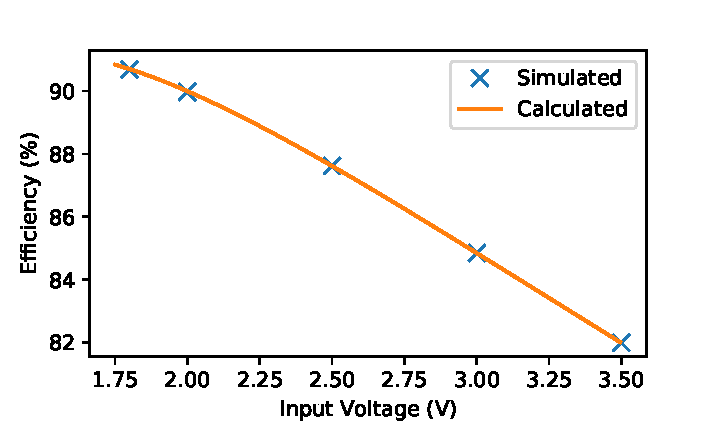
\includegraphics[width=\linewidth]{Figures/eta_VIn.pdf}
 			\caption{Comparison with constant $A = 1$ and $V_{OUT} = 1$.}
 			\label{fig:Comp_VIn}
 		\end{subfigure}
 	\begin{subfigure}{0.49\textwidth}
 		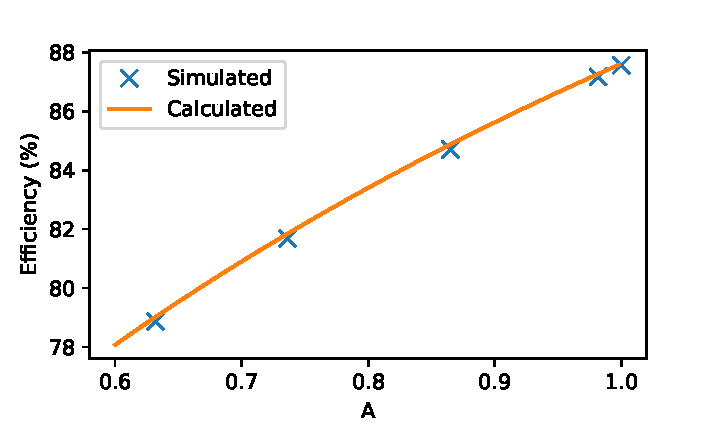
\includegraphics[width=\linewidth]{Figures/eta_A.pdf}
 		\caption{Comparison with constant $V_{IN} = 2.5$ and $V_{OUT} = 1$.}
 		\label{fig:Comp_A}
 	\end{subfigure}
 		\caption{Verification of the calculated efficiency. The simulations were setup to conform to the model assumptions.}
 	\end{figure}
 
 	\section{Steady State Model Usefulness}
 	The usefulness of the model is going to be dependent on how accurate the underlying assumptions are, these will now be discussed. 
 	\subsection{Switch Resistance}
 	The model used assumes constant switch resistance, however the switches are implemented using real transistors. The resistance model for long channel NMOS transistors is,
 	\begin{equation}
 	R_{ON} = \frac{L}{WC_{OX}\mu_N V_{GS}},
 	\end{equation}
 	where $L$ and $W$ are the channel length and width respectively, $C_{OX}$ is the capacitance density of the oxide layer, $\mu_N$ is the carrier mobility, and $V_{GS}$ is the gate voltage relative to the source. This would make $R_{ON}$ dependent on the bottom plate voltage of $C_{Fly}$ (provided $V_G$ is a constant voltage) as $V_{S}$ is going to be determined by the bottom plate voltage. However, if the relative voltage rail configuration is used, as proposed in \cite{Butzen2019}, this can be avoided, and the switches can be modeled as having constant resistance $R_{SW}$. This techniques is used for the PMOS as well again, resulting in a near constant $R_{SW}$.
 	
 	The next portion of this assumption is that switches $S_{B+}$, $S_{B-}$, $S_{T+}$ and $S_{T-}$ have a resistance of 0$\,\Omega$. Clearly, this is not possible, as transistors always have some finite resistance. The motivation behind this design choice is that these transistors switch off and on at a far lower frequency than the other transistors. For example $S_{B+}$ is on for $M+1$ cycles, meaning that it should be sized a factor $\sqrt{M+1}$ larger than the other PMOS transistors.
 	
 	
 	\bibliographystyle{IEEEtran}
 	\bibliography{contBib}
\end{document}